\subsection{Projektorganisation}
\label{sec:Projektorganisation}

Die Vorbereitung der Umsetzung des beschriebenen Projektes beginnt mit der Festlegung der Projektorganisation.
Eine Betrachtung der Projektorganisation ist an dieser Stelle von besonderem Interesse, da die Projektorganisation
den Ordnungsrahmen des Projektes festlegt.
Dieser Ordnungsrahmen dient dazu das zielgerichtete Zusammenwirken
der Projektmitglieder und den reibungslosen Projektablauf sicherzustellen.\footnote{\citet[S.~15]{geiger2009}}

Eine besondere Herausforderung an die Projektorganisation des vorliegenden Projektes ergibt sich hierbei
aus dem angesprochenen Projektumfeld (siehe Abschnitt \nameref{sec:Projektumfeld}). Die Projektmitglieder sind
nicht nur mit der Arbeit am Projekt beschäftigt, sondern zeitgleich auch mit Aufgaben im jeweiligen
Unternehmen, mit anstehenden Prüfungsleistungen und mit Arbeitsleistungen in anderern Modulen.
Die Projektorganisation muss diese Teilung der Arbeitskraft berücksichtigen und daher genügend Flexibilität
besitzen und gleichzeitig eine effiziente Aufgabenverteilung gewährleisten. Darüber hinaus muss
die Zerlegung von Aufgaben in Teilaufgaben und die dezentrale Erarbeitung dieser Teilaufgaben unterstützt werden.

Vor diesem Hintergrund wird die Managementmethode Scrum\footnotemark\ zur Umsetzung der Organisation ausgewählt.
Die Scrum-Methode schafft eine einheitliche Organisationsstruktur, 
indem die Aufgaben des Projekts in Arbeitspakete eingeteilt werden,
die in einem festen Zyklus abgearbeitet werden. Zur Verdeutlichung wird die Scrum-Organisation in \abbildung{Scrum}
dargestellt:

\footnotetext{Scrum ist im ursprünglichen Sinn ein Managementframework, mit dem die die Erstellung von Produkten,
durch Verbesserung und Teilung der Arbeitsaufgaben, effzienter gestaltet werden sollen (vgl. \citet[S.~6]{gloger2013})}

\clearpage
\begin{figure}[htb] 
\centering
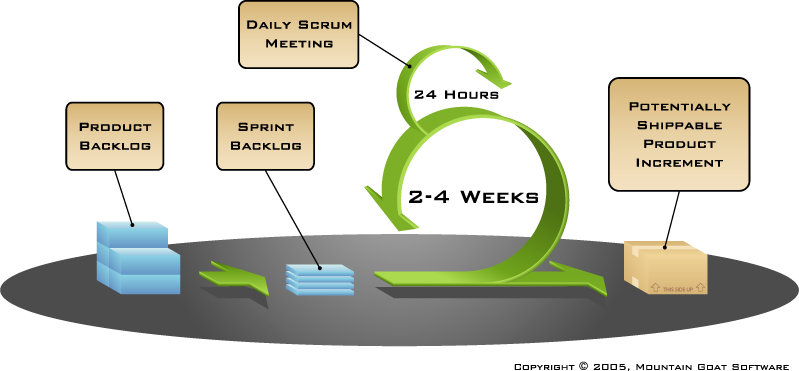
\includegraphics[width=1.0\textwidth]{Scrum.png}
\caption[Scrum-Organisation]{Schematische Organisation eines Projektes mit der Scrum-Methode\protect\footnotemark}
\label{fig:Scrum}
\end{figure}
\footnotetext{Quelle: \url{www.fossa.de}}

Das dargestellte Modell zeigt, dass der Projektinhalt zerteilt und in iterativen Schritten erarbeitet wird. Dieses
Vorgehen schafft, durch die Teilung in zwei iterative Teilprozesse, die nötige Flexibilität der Projektorganisation.
Zum einen ist im Scrum-Modell ein Bearbeitungsprozess vorgesehen
der in zwei bis vier Wochen durchlaufen wird. Dieses Zeitintervall wurde im vorliegenden Projekt für die Erreichung des
nächsten Meilensteins\footnotemark\ vorgesehen. Zum anderen ist ein kleineres Zeitintervall von einem Tag dargestellt, das
genutzt wurde, um kleinere Teilaufgaben auf dem Weg zum nächsten Meilenstein fertig zu stellen.

\footnotetext{Meilensteine stellen elementare Stationen im Verlauf des Projektes dar. Eine genauere Beschreibung
folgt im weiteren Verlauf.}

Durch die Scrum-Organisation konnten kleine Teilaufgaben dezentral bearbeitet werden, ohne die zentrale Erreichung des
nächsten Meilensteins aus den Augen zu verlieren. Eine Projektorganisation, die die aufgezeigten Anforderungen
erfüllt, ist damit definiert.

% \subsubsection*{Möglichkeiten der Projektorganisation}
% \label{sec:MoeglichkeitenProjektorganisation}

% % Scrum ist eine Methode der agilen Softwareentwicklung. Konkret stellt Scrum eine
% % agile Projektmanagementmethode dar. Eine solche Managementmethode behandelt
% % nicht die konkrete Struktur und Art der Zusammenarbeit im Team, sondern
% % beschränkt sich auf den Ablauf des Projektes. Bei einer Projektorganisation nach
% % der Scrum-Methode lassen sich grundsätzlich jeweils drei verschiedene Rollen,
% % Zeremonien und Artefakte unterscheiden. Diese sollen im Folgenden näher
% % beschrieben werden. Die drei zentralen Rollen der Scrum-Methode sind hierbei\ldots

% \subsubsection*{Planung der Projektorganisation}
% \label{sec:PlanungProjektorganisation}

% \subsubsection*{Umsetzung der Projektorganisation}
% \label{sec:UmsetzungProjektorganisation}

% Für eine erfolgreiche Durchführung des Projektes ist es unabdingbar sich vorher
% über die Projektorganisation im Klaren zu sein. Bei der Projektorganisation
% handelt es sich hierbei darum, wie die Entwicklung eines Projektes vonstatten
% gehen soll. Dies bedeutet, dass festgelegt wird, welche Entwicklungsmethodiken
% angewandt werden oder welche Hilfsmittel und Zusatztools eingesetzt werden, um
% das gewünschte Ziel des Projektes möglichst effizient zu erreichen. Ebenfalls
% umfasst dieser Aspekt den Punkt der Kommunikation und Interaktion des
% Projektteams und der einzelnen Projektmitglieder untereinander. Hinzu kommt,
% dass festgelegt wird, wie die einzelnen Meetings der Projektgruppe vonstatten
% gehen und welche Bedingungen erfüllt werden müssen.

% Bei dem großen Umfang und der Vielfalt dieses Projektes ist es notwendig
% flexibel zu sein und somit auf Probleme oder Änderungen und Wünsche des
% Auftraggebers zeitnah reagieren und umsetzen zu können. Um somit die
% Entwicklung agil zu gestalten, entschied man sich in diesem Projekt für die
% Scrum-Methode. Dies ist eine Methodik der agilen Softwareentwicklung und sorgt
% mit sogenannten Scrum-Meetings für regelmäßige Treffen der Projektmitglieder.
% Diese Scrum-Meetings werden immer in gleichen Abständen nach sogenannten
% Sprints gehalten. Die Sprints können hierbei 1 bis 30 Tage lang sein und
% stellen einzelne Iterationsschritte in der Entwicklung der Anwendung dar. Nach
% jeweils einem Sprint, entsteht eine weitere lauffähige Anwendung, aber um die
% Funktionen des letzten Sprints erweitert. Somit wird gewährleistet, dass immer
% eine lauffähige Version zur Verfügung steht und dem Auftraggeber vorgelegt
% werden kann. Nach Ablauf eines Sprints und des darauffolgenden
% Scrum-Meetings,werden weitere Arbeitspakete und Aufgaben an die einzelnen
% Projektmitglieder verteilt, welche in dem folgenden Sprint erledigt werden
% müssen. Durch die kurzen Sprints und häufigen Meetings können so Meinungen,
% Ideen und auch Probleme bei der Umsetzung unter den Projektmitgliedern
% diskutiert und beseitigt werden. Hierbei ist jedes Mitglied gleichberechtigt
% involviert. Trotz dessen können bei der Scrum-Methode folgende drei Rollen
% unterschieden werden:

% \begin{description}
% \item[Der Product Owner] stellt einen Vertreter für den Endkunden dar und
% vertritt somit dessen Wünsche und Bedürfnisse hinsichtlich der Anwendung. Der
% Product Owner trifft somit auch die Entscheidungen bzgl. Kosten und weiterer
% gewünschter Änderungen oder Vorgaben. Die Ergebnisse werden ebenfalls von
% diesem überprüft.
% \item[Der Scrum-Master] dient als Schnittstelle zwischen dem Product Owner und
% dem Scrum-Team und fördert die Zusammenarbeit. Ebenfalls sorgt er dafür, dass
% das Scrum-Team nach den Regeln der Scrum-Methode arbeiten.
% \item[Das Scrum-Team] ist für die Entwicklung und Implementierung der
% gewünschten Anwendung zuständig. Es handelt eigenständig und organisiert somit
% sich und die Vorgehensweise in großem Maße selbst.
% \end{description}

% Ebenfalls zu erwähnen ist, dass ein Product-Backlog ein vom Endkunden
% definierter Katalog ist, welcher die Anforderungen des Kunden , nach Priorität
% und Wichtigkeit sortiert, enthält. Die Anforderungen des Product-Backlog werden
% dabei in ein sogenanntes Sprint-Backlog übertragen, welches bei den Sprints als
% Vorlage für die zu erfüllenden Aufgaben dient. Nach jedem Sprint werden die
% erzielten Ergebnisse, unabhängig von der erreichten Vorgaben, in einem Sprint
% Review dokumentiert und an den Product Owner zur Einsicht übergeben.

% In folgender Abbildung wird der Scrum-Prozess nochmals visuell dargestellt:

% Nach einer kurzen Einführung in die agile Softwareentwicklung kann nun gesagt
% werden, dass das Projektteam in diesem Projekt agil entwickelt hat. Dazu wurde
% eine Sprintdauer von einer Woche angesetzt. Nach dieser Woche fand immer ein
% Scrum-Meeting statt, in der die Erkenntnisse und Ergebnisse der einzelnen
% Projektmitglieder reflektiert wurden. Für die einzelnen Scrum-Meetings sind
% ebenfalls Gesprächsprotokolle erstellt worden, auf die im Nachhinein
% zugegriffen werden kann (siehe Anhang). Bei besonders komplexen Problemen
% während der Entwicklung der Anwendung, wurde auf die Methode des Pair
% Programming zurückgegriffen. Dies bedeutet, dass mehrere Mitglieder
% gleichzeitig und zusammen an einem Rechner an einem Implementierungsproblem
% arbeiten. Dadurch konnten komplexe Probleme schneller und effizienter beseitigt
% werden, da sich die Teammitglieder während des Arbeitens direkt austauschen
% können. Zum Schluss jedes Scrum-Meetings wurden ebenfalls neue Arbeitspakete an
% die Gruppenmitglieder verteilt.

% Die Verwaltung der Arbeitspakete wurde dabei durch ein zusätzliches Tool
% realisiert, welches sich PHProjekt nennt. Dieses Tool ist ein webbasiertes
% Ticketsystem, welches es ermöglicht Arbeitspakete einzelnen Gruppenmitgliedern
% zuzuweisen und deren einzelne Status anzeigen zu lassen. Ebenfalls ist es hier
% möglich Prioritäten und Dauer zu definieren, um die wichtigsten Arbeitspakete
% zu kennzeichnen und eine Frist zur Erledigung zu setzen.

% Um die einzelnen Programmversionen, welche nach den Sprints entstehen, zu
% verwalten, wurde die Versionsverwaltung Github eingesetzt, welche ebenfalls
% webbasiert arbeitet. Hiermit ist es möglich Abspaltungen von einer bestehenden
% Programmversion zu erzeugen und diese zu bearbeiten und nach Abschluss wieder
% der Stammversion hinzuzufügen. So kann gewährleistet werden, dass immer eine
% funktionsfähige Version zur Verfügung steht, da isoliert von der Stammversion
% gearbeitet und entwickelt wird.